\chapter{Osobnost Karla Makoně}

%\section{Životopis}

Pokusím se přiblížit, co za člověka Karel Makoň byl, tím, že převyprávím jeho
život podle toho, jak a s~jakými důrazy ho podává on sám. Je to příběh plný
zázraků, což odpovídá tomu, že Makoň na svém životě demonstruje působení
zázračného tažení Božího. Nic mu to ale aspoň v~mých očích neubírá na
pravdivosti.

Stať o Makoňově životě čerpá z~jeho knihy Umění žít\cite{KaMaUZ} a ze záznamů nahrávek.
Některá fakta o Makoňově životě opírám pouze o ústní svědectví pamětníků.

\section{Poznávání správného}

Karel Makoň se narodil 12.12.1912 v~nemocnici Plzeň-Bory do rodiny z~Ošelína,
viz matriční záznam na obr.~\ref{fig:matrika}\footnote{Matriční záznam je
dostupný na adrese
\href{https://www.portafontium.eu/iipimage/30072742/plzen-138-0230-n}{portafontium.eu/iipimage/30072742/plzen-138-0230-n}.}. Jeho otec osm měsíců
nato zemřel na tuberkulózu a Karel sám dostal zánět do levého ramene.\footnote{Umění žít, str. 87} Ten dospěl
do takového stádia, kdy lékař doporučil amputaci ruky. Matka amputaci odmítla a tak
započala první fáze Makoňovy duchovní formace. Rameno bylo nutno operovat.
Jelikož se ještě nepoužívala transfúze, musela se operace provádět na
několikrát, protože jinak by dítě vykrvácelo. A kvůli Makoňově útlému věku a
stavu tehdejší anesteziologie musely operace probíhat za vědomí. Dítě bylo
vystaveno takové bolesti, že se naučilo vystupovat z~těla.\footnote{Umění žít,
str. 24} Toto se podle
Makoňových slov opakovalo čtrnáctkrát,\footnote{Umění žít, str. 27} což malého Karla Makoně nezvratně
změnilo.

\begin{figure}[htpb]
\includegraphics[scale=0.74, angle=90]{rc/matrika.png}
\caption{%
  Záznam Makoňova narození, křtu a sňatku z~matriky Plzně 3
}
\label{fig:matrika}
\end{figure}

Ve stavech mimo tělo, kdy necítil bolest, se setkával s~něčím, co nazývá
,,žlutým světlem``\rref{86-04A-Brno\_8.2.1986}{12:25}.  Důsledkem bylo, že dítě začalo samovolně rozlišovat, co je
  správné, a bylo vnitřně puzeno správné následovat. Správné od nesprávného dokázal
Makoň rozpoznat, ale neměl schopnost správné řešení situace sám
vymyslet\rref{85-35A}{24:16}. Důvěřoval
matce a tak ji častoval otázkami, jak se má zachovat. Mnohokrát pak její návrh
odmítl s~tím, že tohle dělat nebude, a chtěl dostat návrh jiný. Jeho
matce se zdálo, že dítě si svévolně vybírá a matku trápí\rref{83-01B}{31:25}.

V~období raného dětství vyčníval Karel Makoň nejen svým příklonem ke správnému, ale
také blízkým vztahem ke zvířatům. Aby se operované rameno neporanilo, měl
Karel Makoň zapovězeno hrát si s~jinými dětmi\footnote{Umění žít, str. 5}. Trávil proto svůj volný čas
v~předškolním věku téměř výhradně o samotě se zvířaty, obzvláště s~husami.
Naučil se rozumět jejich řeči a ony ho přijaly mezi sebe jako jednoho
z~nich\footnote{Umění žít, str. 33}, srovnej s~dílem Konrada
Lorenze\cite{lorenz1949redete} a tradicí o Františkovi z~Asisi\cite{thompson2012francis}.

Makoň poznal, že husy ve stavu spánku nejsou nečinné, nýbrž žijí intenzivním
životem na jiné úrovni. Vzaly ho oďobáváním na správných místech s~sebou a on
s~nimi prožíval ,,stav zvířecího ráje``, kde bylo přítomno celé hejno, ale
nikoliv v~tělech, nýbrž bez nich. Prožívaly pospolitost, viděly na sobě, jaké
mají neduhy a co je potřeba k~jejich překonání.\footnote{Umění žít, str. 35}

Poznání skutečného zvířecího ráje, ke kterému nemá běžný člověk přístup, a
puzení vyhnout se nesprávnému, vedly Karla Makoně k~pevnému rozhodnutí vystříhat
se veškerého ,,pohlavního života``, jak sexuální aktivitu konzistentně
nazývá.\footnote{Umění žít, str. 53}

Jeho matka a obzvláště babička Karla Makoně vedly ke zbožnému katolickému
životu. Musel se pravidelně modlit a chodit do kostela.\footnote{Umění žít, str.
54} Vysvětlovaly mu to tak,
že nebude-li toho činit, přijde do pekla, zatímco když bude, dojde do nebe, kde
se bude věčně dívat na Boží tvář. Makoňovo inspirované rozpoznání správného a
nesprávného mu neomylně radilo, že tohle správné není a tak nevěřil. Do nebe se
dostat nechtěl, protože takto popsané mu připadalo jako ukrutná nuda, a modlitby
prováděl jen matce a babičce k~vůli, neboť rozpoznával jako správné řídit se
jejich přáním\rref{kotouc-I01-81-82-Plzen-02-b}{45:36}.

Ve škole prožíval Karel Makoň těžké loučení se zvířecím světem a sžívání s~tím
lidským. Poznával ale jak v~matce tak v~učitelích autority, takže se převychovat
nechal.\rref{82-15}{01:05:23} Vedlo to nakonec k~tomu, že Karel Makoň si v~životě vytvořil jedinou
skutečnou lásku, a tou byly přírodní vědy. Toužil stát se přírodovědcem víc než
po čemkoliv jiném\rref{85-31B}{40:59}. Když ho pak rodinná finanční situace donutila se tohoto snu
vzdát, ztratil svoji jedinou lásku a s~tím jakoby sama sebe.
Tímto dospěl do druhého zlomu po operacích ramene\footnote{Umění žít, str. 60}.

\section{Modlitba za lásku}

Makoň byl nucen studovat ekonomii, a aby aspoň nějak ukojil touhu po přírodních
vědách, chodil si číst přírodovědné knihy do knihovny. Při jedné takové
příležitosti namátkou otevřel knihu a oči mu padly na větu, která ho uchvátila a
strhla do prvního vytržení. Stálo tam, že tento život je mostem do
Věčnosti\footnote{Přesné znění citátu se liší. V~Umění žít na straně 72 se
uvádí \textit{,,Nežijeme na tomto světě, abychom tu něco provedli a zemřeli,
nýbrž proto, abychom se pomocí pozemského života stali vědomě nesmrtelnými
bytostmi,``} kdežto v~nahrávce \texttt{77-03A-Zlin-77-3-b} od pozice 44:53 se
uvádí \textit{,,tento tvůj život je mostem do věčnosti.``}}.

Onen zdánlivě banální zážitek poskytl Makoňovi niterné setkání se svojí věčnou
podstatou, ovšem jen chvilkově. Tehdy absolutně ztratil zájem o všechny světské
záležitosti. Matka ho musela několik dní nutit do jídla a spánku, studiu se
věnoval s~extrémní nechutí a jen kvůli svým blízkým. Jediným jeho zájmem se
stalo spojení s~Věčností, které zakusil v~knihovně.

Tehdy si vzpomněl na svoji katolickou výchovu a obrátil se na kněze s~prosbou o
generální zpověď\footnote{Umění žít, str. 76}. Jaký byl knězův údiv, když ho Makoň žádal o rozhřešení za to,
že nežil dosud jen pro Boha! A o kolik větší byl ještě jeho údiv, když při
dalším setkání Makoň tvrdil, že nezhřešil. Konsternovanému knězi to vysvětlil
tak, že nemůže hřešit, i kdyby chtěl, protože pociťuje přítomnost Boží a ta mu
žádný hřích nedovolí.\rref{89-06B}{26:42}

Vytržení, nebo jak je sám nazývá \textit{,,extaze``}, zažíval opakovaně. Pokaždé
zakoušel nevyhnutelnost vlastního zániku a pokaždé utekl. Poté si vždy
%v~nich zažíval jistotu vlastního zániku a s~hrůzou utekl a pokaždé si pak
předsevzal, že příště již neuteče\footnote{Umění žít, str. 101}. Stanovil si nejpřísnější řeholi, jaká ho
napadla, a modlil se bez ustání výhradně za to, aby dokázal Boha více milovat,
neboť cítil, že k~Němu chová lásku zcela neadekvátní Boží vznešenosti. Ba
pociťoval to tak, že vlastně vůbec žádné lásky není sám
schopen\rref{kotouc-B01-70-08-29-Zlin-moderni\_tendence\_v\_oblasti\_poznani-b}{38:26}.

Toto trvalo devět let a vyústilo do dalšího, zdaleka nejzávažnějšího zlomu
v~Makoňově životě.

\section{Koncentrační tábor}

Datum sedmnáctého listopadu máme spojeno se Sametovou revolucí, kde výraznou
roli hráli demonstrující studenti. V~týž den roku 1939, tedy
přesně půl století před tím, byly nacisty uzavřeny české vysoké školy a studenti
deportováni k~likvidaci. Toho se stal obětí i Karel Makoň\footnote{Umění žít,
str. 42}. Je trochu ku podivu,
že byl i on deportován, neboť při zásahu nacistů nebyl ve škole. Došel již do
prázdné budovy později a odvedené spolužáky sám vyhledal a přihlásil se k~nim.
% TODO: doložit
Poté dokonce vyvolávali jeho jméno, jako jednoho z~těch, kteří měli být
propuštěni, neboť měl už fakticky studium za sebou. Dostal ovšem před tím ránu
pažbou do hlavy a dočasně ztratil sluch, takže nevěděl, že je
vyvoláván\rref{89-35B}{03:07}.

V~koncentračním táboře nastalo pro Makoně naprosté peklo. Snad k~tomu přispěla
zakrnělá ruka\footnote{Toto je moje domněnka.}, že Makoň schytával bití,
šikanu a ústrky více než ostatní spoluvězni. Ti se nejednou podivili, že
kdykoliv se rozdávaly rány, Makoň jako by se tam zákonitě připletl a schytal
ještě víc.

Snad ještě horší než faktické strádání násilím, hladem, nečistotou a vůbec
podmínkami k~živoření byl pro Makoně fakt, že po devíti letech,
kdy se usilovně modlil za větší lásku k~Bohu a zachovával absolutní čistotu a
věrnost, s~ním duchovně zakrnělí lidé mají právo nakládat jako s kusem hadru.
Cítil se Bohem opuštěn a zrazen. A dodává, že kdykoliv si toto pomyslel, hned tu
byl kopanec nebo políček od dozorce\rref{80-02A}{29:15}.

Tragická epizoda vyvrcholila 21. listopadu 1939 po čtyřech dnech krutého utrpení. Vězňové
v~koncentračním táboře měli zapovězeno sledovat nacisty, jak vraždí některého
z~jejich spoluvězňů. Makoně ovšem jeden z~Němců právě při tomto přistihl. Právě
dobíjel jednoho vězně a vyzval Makoně, aby zůstal na místě, že hned po něm je na
řadě on. Vyzbrojen svými předchozími zážitky a devítiletou disciplínou, dokázal
Karel Makoň v~dozorci nevidět zrůdu, ale posla Božího. Klidně, bez slovních deklarací,
složil život do Božích rukou. Gestapák se už napřahoval k~zasazení rány, když
v~tom hrůzou zbledl a obrátil se na útěk\rref{kotouc-A01-c}{26:52}.

Karel Makoň v~této chvíli mystické smrti, kdy vnitřně zemřel, ještě než zemřel
fyzicky, podle svých slov obdržel najednou poznání významu celé situace. Poznal,
proč je v~koncentráku, proč tam je každý z~ostatních, za jakých podmínek se
odtamtud dostane, a především obdržel poznání celé symboliky biblického textu,
katolické tradice i jiných svatých písem.

Od tohoto momentu se Makoň vyvázal z~veškerého utrpení. Jedl i pil dále stejně
jako ostatní, ale příděly mu bohatě stačily. Zažíval naprostou svobodu.
Procházel volně bezi baráky, hlídky ho nikdy nespatřily. Všem svým spoluvězňům
kázal slovo Boží a osvětloval jim, jak se i oni mohou z~utrpení
vyvázat\rref{85-36B-gt\_do\_475}{33:31}.

\section{Život v~Boží přítomnosti}

Ve vydávání svědectví o tom, že lze dosáhnout vědomého spojení s~Bohem, vytrval
Makoň i po propuštění z~koncentračního tábora. Zasvětil celý zbytek života tomu,
aby svoje poznání předal dál a aby pomohl ostatním lidem
naplnit smysl života, ovšem bez tak těžkých krizí, jaké sám
zažíval\footnote{Mozaika mystického života Karla Makoně, str. 10}. Napsal
dvacet sedm knih a dvacet osm jich přeložil a komentoval. Všechny jsou dostupné
na internetové stránce \href{http://makon.cz/}{makon.cz}.

Krom psaní pravidelně přednášel v~úzkém kruhu přátel na~různých místech
Československa. Měl skupinku posluchačů především ve Zlíně, v Plzni a v Praze.
Tyto spontánní přednášky, které se odehrávaly většinou u některého účastníka
doma nebo na několikadenním výjezdu, někteří účastníci nahrávali na
magnetofonové pásky. Z~toho vznikl archiv více než tisíce hodin záznamu. Jeho
zpracování a zpřístupnění je tématem mojí informatické disertační
práce\cite{kruuza2021iterativni}. Nahrávky jsou dostupné na adrese
\href{http://radio.makon.cz/}{radio.makon.cz}.

Budil zájem St.B., která ho též vedla jako spolupracovníka, viz str. 176
plzeňského archivu bezpečnostních
složek\footnote{\href{https://www.abscr.cz/data/pdf/knihy//PLA/PLA\_8.pdf}{abscr.cz/data/pdf/knihy//PLA/PLA\_8.pdf}},
zde na obr.~\ref{fig:orel}. Jeho složku jsem nedokázal dohledat, nicméně podle
ústních svědectví se to s~jeho spoluprací s~St.B. mělo takto: Když se vracel
z~KZ, dostal posudek od nacistů, kde se o něm tvrdilo, že spolupracoval
s~americkou tajnou službou. Na základě toho ho Státní bezpečnost vedla
v~patrnosti. Kontakt s~ní měl pro Makoňovo působení i pozitivní dopady. Ve
večerní škole Makoň učil policisty i příslušníky St.B. a díky tomu jich mnoho
osobně znal a dostával varování, když měl být např. sledován. O~žádné reálné
kolaboraci nemám informace, naopak všechna svědectví se shodují, že nebyla.

Občanským zaměstnáním byl Makoň středoškolským učitelem, z~čehož také plyne
tradice mezi jeho příznivci, nazývat ho profesorem. Pro doklad jeho působení na
Střední škole ekonomické v~Plzni viz přílohu~\ref{apx:almanach}. Oženil se (viz matriční
doklad na obr.~\ref{fig:matrika}) a měl tři děti.
%TODO: kdy zemřela manželka?
Zemřel 24. října 1993, rok po svojí poslední přednášce. Jeho život byl protkán
zázračnými událostmi, z~nichž některé si získaly punc významnosti. Ty jsou
sepsány v~knížce Mozaika mystického života Karla Makoně\cite{kaliban2002mozaika}, kterou na
jeho památku jeho následovníci po jeho smrti sepsali.

\begin{figure}[htpb]
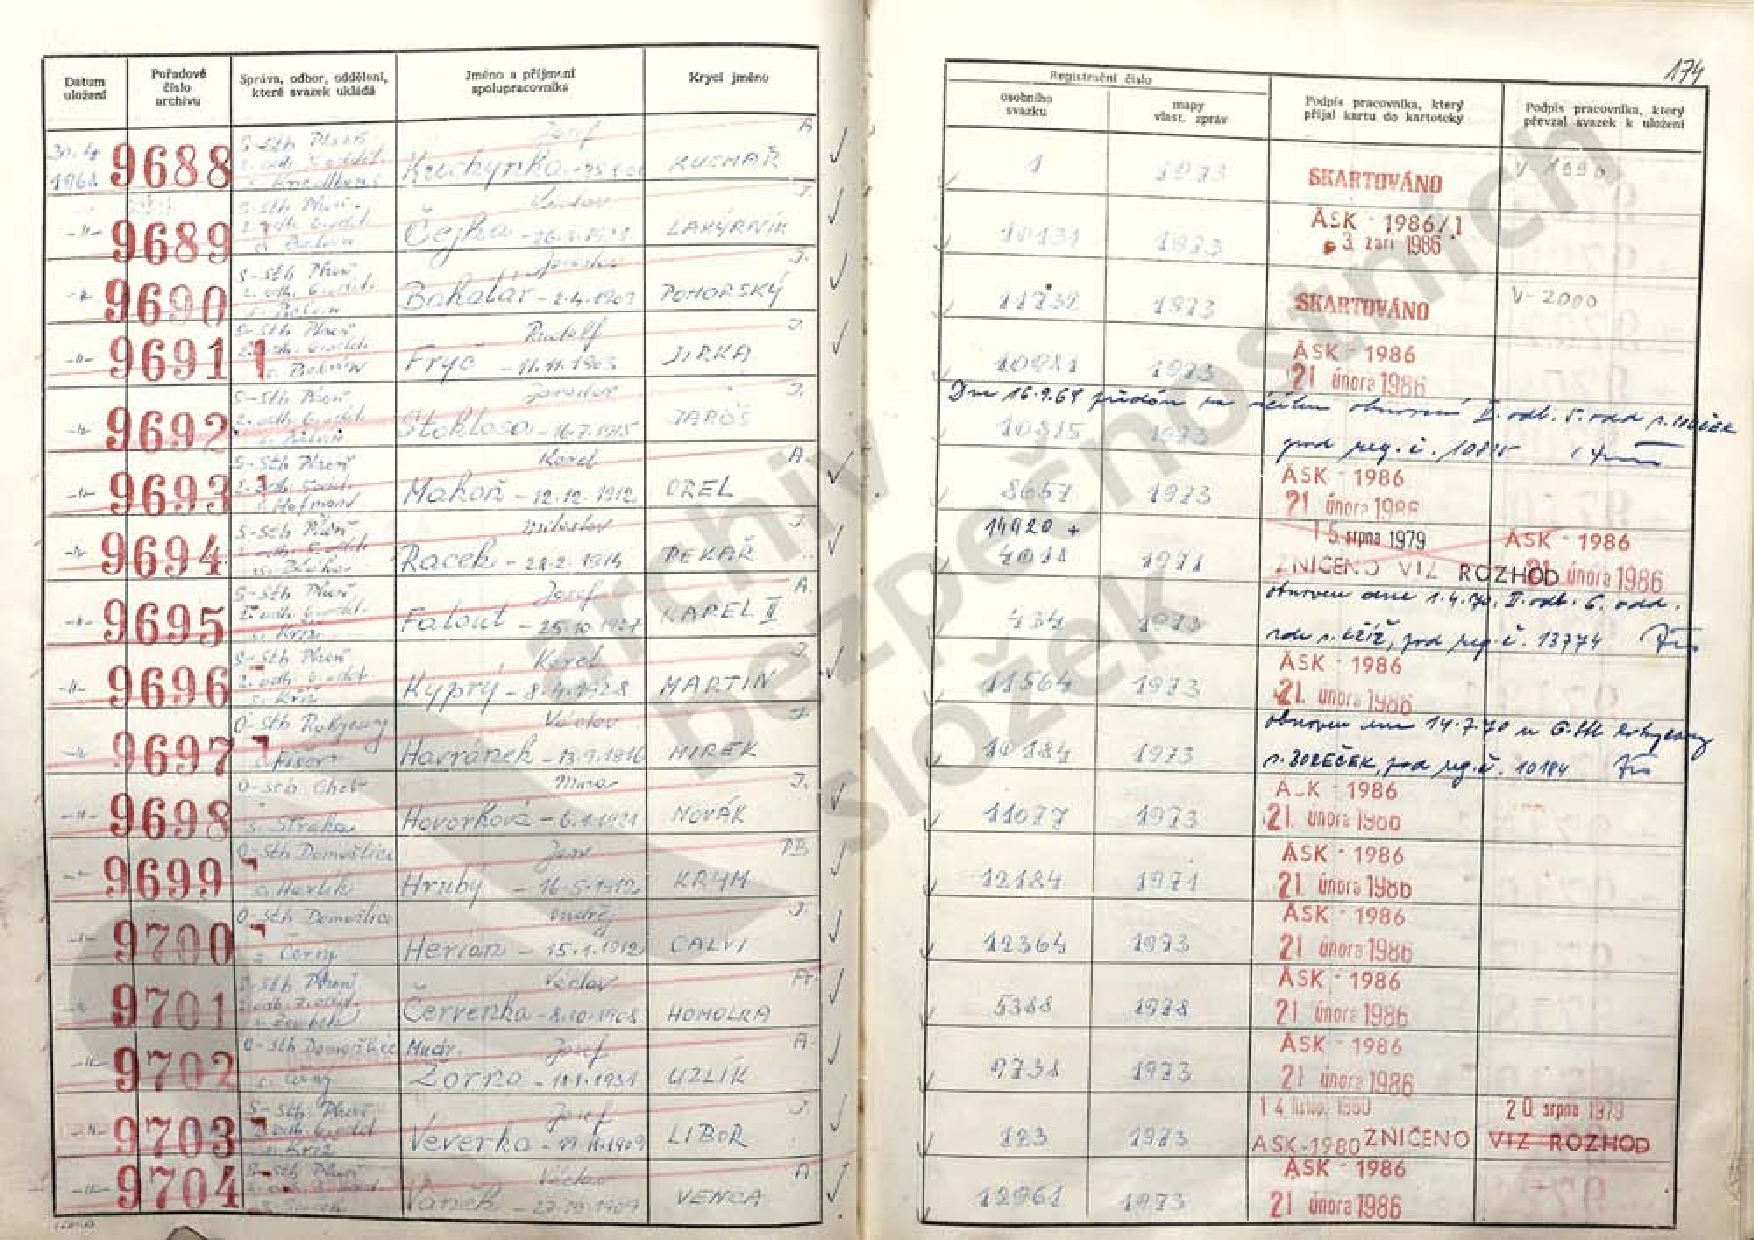
\includegraphics[scale=0.68, angle=90]{rc/orel.pdf}
\caption{%
  Karel Makoň v~seznamu spolupracovníků Státní bezpečnosti
}
\label{fig:orel}
\end{figure}

%\section{Anekdoty}
%
%Příběh o tom, jak Karel Makoň překonal smrt v~koncentračním táboře a jak byl na
%tuto mezní událost připravován, nám přibližuje, jak se z~něho stal člověk,
%kterým byl po celý zbytek života. Jak ale s~touto hřivnou hospodařil? Jaký byl
%jako člověk? Na tuto otázku mohu sám odpovědět jen těžko, sám Makoně nezaživ.
%
%V~jeho řeči rozpoznávám přirozenou autoritu a humor. Jeho žáci, které znám, ho
%často citují a je znát, že pro ně byl nezpochybnitelnou autoritou a že ho
%nesmírně milovali. Mnohdy se vyprávění koncentruje na zázračné události, který
%ten který svědek s~Makoněm zažil. Jeden z~výrazných Makoňových žáků svědčí o
%tom, že s~Makoněm bylo veselo. Říká, že se někdy smáli tak, až ho prosil, ať už
%té legrace nechá, jinak že snad tolik veselí ani nevydrží. Tomu nasvědčuje i
%fakt, že Makoň byl alergický na takzvané \textit{,,smutné svaté``}.
%
%\subsection{Záhrobí}
%
%Karel Makoň svoji manželku přežil. Na sklonku života trpěla bolestmi a Makoň ji
%naučil dechovými technikami opouštět tělo. Když tedy přešla práh smrti, měla již
%za sebou jistý trénink a na onom světě žila poněkud uvědomělejším životem. Makoň
%s~ní pak vedl velmi bohatou a dlouhodobou komunikaci, která mu zprostředkovala
%kromobyčejně detailní informace o záhrobním životě.
%
%Koluje legenda, že ve dvanáct hodin a
%dvanáct minut, ovšem sám Karel Makoň zmiňuje v~Umění žít\cite{KaMaUZ}, bylo to
%podle záznamu jeho otce v jednu hodinu a devatenáct minut v noci.
